%%
%% Structure of this section
%%
%%  3.1 define basics, abstraction of stream processing
%%    - Def. data items, data streams,...
%%    - data flow vs. control flow => Bezug zu Anytime
%%    - Warum keine "Meta-Daten" (bisher)
%%
%%  3.2 Umsetzung/Modellierung in Form der Stream-API
%%    - Abbildung der Konzepte aus 3.1 auf "Java Welt"
%%  
%%  3.3 Example Runtime for RapidPrototyping, Debugging
%%    + Ausblick auf section 4 => streamplugin + runtime f�r RapidMiner
%%
%%
\section{\label{sec:abstraction}An Abstract Stream Processing Model}
In this section we introduce the basic concepts and ideas that we
model within the \streams framework. This mainly comprises the data
flow (pipes-and-filters \cite{softwarePatterns}), the control flow
(anytime services) and the basic data structures and elements used for
data processing. The objective of the very simple abstraction layer is
to provide a clean and easy-to-use API to implement against. The
abstraction layer is intended to cover most of the use cases with its
default assumptions whereas any special use cases can generally be
modelled using a combination of different building blocks of the API
(e.g. queues, services).

\subsection{\label{sec:notation}Data Streams and Items}
We consider the case of continuous streaming data being modeled as a
sequence of data items. Throughout this work, we will denote a {\em
  data stream} by $D$ and a family of such streams as $D_l$. A data
stream $D$ is a sequence
\begin{displaymath}
  D = \langle d_0,d_1,\ldots,d_i,\ldots \rangle
\end{displaymath}
of data items $d_i$. Let $A = \{A_1,\ldots,A_p\}$ be a set of
attributes, then a data item $d_i$ is a function mapping attributes to
values of a domain associated with each attribute. In database
notation, each $d_i$ is a tuple of $M^p = M_{A_1} \times\ldots\times
M_{A_p}$ for sets $M_j$. The $M_j$ can be any discrete sets of a fixed
domain as well as $M_j \subseteq \mathbb{R}$. The values of each data
item are further denoted by $d_i(k)$, i.e.
\begin{displaymath}
  d_i = ( d_i(A_1),\ldots,d_i(A_p) ).
\end{displaymath}

The index $i$ may reflect some time unit or a (monotonically
increasing) time-like dimension, constituting the sequence of
tuples. For $p=1$ and $M_1 = \mathbb{R}$ this models a single value
series with index $i$.


%
%. The {\em data items} $s_i$ are tuples of
%$M^p$ with $p \ge 1$ where $M^p = M_1 \times \ldots \times M_p$ for
%any sets $M_j$. 
%

\subsection{\label{sec:basics}Stream Processes and Processors}
A stream provides access to single {\em data item} (also referred to
as instances, events or examples) which are sequentially processed by
one or more processing units. As noted above, each data item
represents a tuple, i.e. a set of ({\em key}, {\em value}) pairs and
is required to be an atomic, self contained element. Data items from a
stream may vary in their structure, i.e. may contain different numbers
of ({\em key}, {\em value}) pairs (e.g. for sparse elements).

%A data item {\em may} correspond to the notion of an example known
%from RapidMiner, but this is not always the case as we will show in
%the use case of the FACT telescope data in Section \ref{sec:usecases}.


\begin{figure}[h!]

  \begin{center}
{\footnotesize
    \begin{tikzpicture}[scale=0.8]
      \node[cylinder,inner sep=2ex,draw=black!60] at (0,0) {\textsf{Data Stream}};
      
      \node[fill=red!8,inner sep=1ex,draw=red!40] (a) at (2.5,0) {A};
      \node[fill=red!8,inner sep=1ex,draw=red!40] (b) at (3.5,0) {C};

      \node at (5,1.3) {\textsf{Process}};
      \draw[dashed] (4,-1) -- (11,-1) -- (11,1) -- (4,1) -- (4,-1);
      
      \node[inner sep=2ex,draw=black!60,fill=black!10] (proc) at (5.5,0) {\textsf{Processor}};

      \node[circle,fill=red!8,inner sep=1ex,draw=red!40] (a) at (7.5,0) {a};
%      \node[circle,fill=green!8,inner sep=1ex,draw=green!40] (b) at (8.5,0) {c};

      \node[inner sep=2ex,draw=black!60,fill=black!10] (proc) at (9.5,0) {\textsf{Processor}};
      \node[circle,fill=blue!8,inner sep=1ex,draw=blue!40] (a) at (11.5,0) {a};
      \node[circle,fill=blue!8,inner sep=1ex,draw=blue!40] (a) at (12.5,0) {c};

      \draw[->,draw=black!40,very thick] (0,-1.25) -- (12,-1.25);
    \end{tikzpicture}
}
    \caption{\label{fig:pipeline}The general pipeline model for data processing.}
  \end{center}
\end{figure}

A {\em data stream} is essentially a possibly unbounded sequence of
data items. In the pipeline model, a {\em processor} is some
processing unit that applies a function or filter to a data item. This
can be the addition/removal/modification of ({\em key}, {\em value})
pairs to the current item or an update of some model/state internal to
the processor. Then the outcome is delegated to the subsequent
processor for further computation. Figure \ref{fig:pipeline}
illustrates an abstract data process flow following the widely
accepted pipes-and-filters pattern.

\subsubsection*{Functional Representation of Processes}

As a more abstract concept, each processor is a function $f: M^p\times
C \rightarrow M^{p'}\times C'$, where $C$ is some (global) state. This
state $C$ exhibits the fact, that processors may make use of a state,
e.g. a learnt model. A list of processors $f_1,\ldots,f_m$ can now be modeled as a
sequence of function applications
\begin{displaymath}
  f = f_m \circ \ldots\circ f_1.
\end{displaymath}
%Note here, that the $f_i$ {\em may} maintain an internal state or
%produce side effects, so the term {\em function} does not refer to
%pure functions in the mathematical or functional programming sense.

Processors are applied to single data items. A list of processors is
wrapped into a {\em process}, which handles a stream of data
(sequence). A process $P$ can be defined as a function on sequences,
built upon a list of processors
\begin{eqnarray*}
  P &=& f_m \circ\ldots\circ f_1 \\
  \langle d_0,d_1,\ldots \rangle &\mapsto& \langle P(d_0,C_0),P(d_1,C_1),\ldots \rangle
\end{eqnarray*}
for an initial state $C_0$ of the process. The implicit sequence of
states $C_0,C_1,\ldots$ represents the evolving state of the process.


\subsubsection*{Using multiple Processes}
In the \streams framework, a process is an active component that
reads from a stream and applies all inner processors to each data
item. The process will be running until no more data items can be read
from the stream. Multiple streams and processes can be defined and
executing in parallel.  For communication between processes, the environment
provides the notion of {\em queues}. Queues can temporarily store a 
limited number of data items and can be fed by processors. They do
provide stream functionality as well, which allows queues to be read
from by other processes.

Figure \ref{fig:queues} shows two processes being connected by a queue.
The processor $f_i$ in the first process is a simple {\em Enqueue} function
that pushes a copy of the current data item into the queue $Q$. The
second process constantly reads from this queue, blocking while the queue
is empty.

\begin{figure}[h!]
  \begin{center}
{\footnotesize
    \begin{tikzpicture}[scale=0.8]
      \node[cylinder,inner sep=2ex,draw=black!60] at (-1,0) {\textsf{Stream} $D$};

      \node at (3,1.1) {\textsf{Process} $P_1$};
      \draw[dashed,draw=black!40] (1.75,-0.75) -- (7.25,-0.75) -- (7.25,0.75) -- (1.75,0.75) -- (1.75,-0.75);

      \node[fill=red!8,inner sep=0.75ex,circle,draw=red!40] (a) at (1.5,0) { $d$ };
      
      \node[inner sep=1ex,draw=black!60,fill=black!10] (proc) at (2.5,0) { $f_1$ };

      \node (crc) at (3.25,0) { $\circ$ };

      \node[inner sep=1ex,draw=black!60,fill=black!10] (fe) at (4.0,0) { $f_i$ };

      \node (crc) at (4.75,0) { $\circ$ };

      \node at (5.25,0) { $\cdots$ };     

      \node (crc) at (5.75,0) { $\circ$ };

      \node[inner sep=1ex,draw=black!60,fill=black!10] (proc) at (6.5,0) { $f_k$ };

      \node[cylinder, inner sep=1.5ex, draw=black!60] (q) at (4.0,-2.5) {\textsf{Queue} $Q$};

      \draw[draw=black,->] (fe.south) -- (q.north);


      \node at (8,-1.4) {\textsf{Process} $P_2$};
      \draw[dashed,draw=black!40] (6.75,-3.25) -- (10.75,-3.25) -- (10.75,-1.75) -- (6.75,-1.75) -- (6.75,-3.25);

      \node[fill=red!8,inner sep=0.65ex,circle,draw=red!40] (a) at (4.0,-1.25) { $d'$ };

      \node[fill=red!8,inner sep=0.65ex,circle,draw=red!40] (a) at (6.4,-2.5) { $d'$ };

      
      \node[inner sep=1ex,draw=black!60,fill=black!10] (proc) at (7.5,-2.5) { $h_1$ };

      \node (crc) at (8.25,-2.5) { $\circ$ };

      \node at (8.75,-2.5) { $\cdots$ };      

      \node (crc) at (9.25,-2.5) { $\circ$ };

      \node[inner sep=1ex,draw=black!60,fill=black!10] (proc) at (10,-2.5) { $h_n$ };

    \end{tikzpicture}
}
  \end{center}
  \caption{\label{fig:queues}Two Processes $P_1$ and $P_2$ communicating via queues.}
\end{figure}

\bigskip

These five basic elements ({\em stream}, {\em data item}, {\em
  processor}, {\em process} and {\em queue}) already allow for
modelling a wide range of data stream processes with a sequential and
multi-threaded data flow.
%This contrasts to the current RapidMiner execution model, where each
%operator within a process is executed only once (not counting loops as
%within a cross validation).
%This simple {\em data flow} view serves as the basic data-driven
%exectuion model. 
Apart from the continuous nature of the data stream source, this model
of execution matches the same pipelining idea known from tools like
RapidMiner, where each processor (operator) performs some work on a
complete set of data (example set).

\subsection{Data Flow and Control Flow}
A fundamental requirement of data stream processing is given by the
{\em anytime paradigm}, which allows for querying processors for their
state, prediction model or aggregated statistics at any time. We will
refer to this anytime access as the {\em control flow}.  Within the
\streams framework, these anytime available functions are modeled as {\em
  services}. A service is a set of functions that is usually provided
by processors and which can be invoked at any time. Other processors
may consume/call services. 

This defines a control flow that is orthonogal to the data flow. Whereas
the flow of data is sequential and determined by the data source, the
control flow represents the anytime property as the functions of services
may be called asynchronuous to the data flow.
Figure \ref{fig:control} shows the flow of data and service access.

Examples for services my be classifiers, which provide functions for
predictions based on their current state (model); static lookup
services, which provide additional data to be merged into the stream
or services that can be queried for current statistical information
(mean, average, counts).

\begin{figure}[h!]
  \begin{center}
    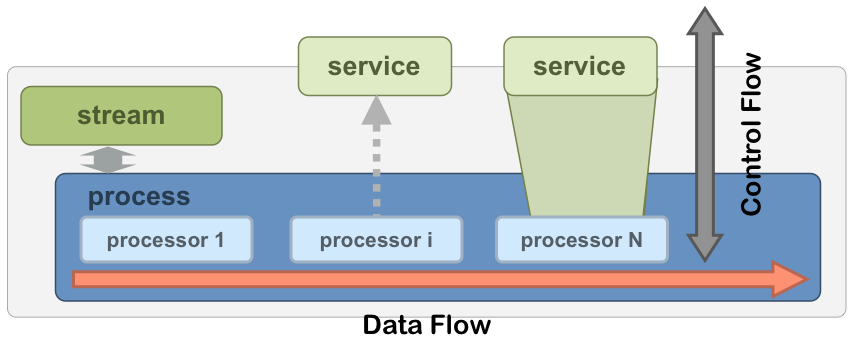
\includegraphics[scale=0.35]{graphics/data-control-flow.png}
  \end{center}
  \caption{\label{fig:control}Orthogonal {\em data} and {\em control
      flow}. Processors may use services as well as export
    functionality by providing services.}
\end{figure}

\subsubsection*{Service References and Naming Scheme}
In order to define the data flow as well as the control flow, a naming
scheme is required. Each service needs to have an unique identifier assigned
to it. This identifier is available within the scope of the experiment and
will be used by service consumers (e.g. other processors) to reference that
service.

At a higher level, when multiple experiments or stream environments are running
in parallel, each experiment is associated with an identifier by itself. This
imposes a hierarchical namespace of experiments and services that are defined
within these experiments. The {\em streams} library constitutes a general
naming scheme to allow for referencing services within a single experiment
as well as referring to services within other (running) experiments.

A simple local reference to a service or other element (e.g. a queue) is 
provided by using the identifier (string) that has been specified along with
the service definition. Following a URL like naming format, services within
other experiments can be referenced by using the experiment identifier and
the service/element identifier that is to be referred to within that experiment,
e.g.
\begin{displaymath}
  \mbox{\ttfamily //experiment-3/classifier-2}.
\end{displaymath}
Such names will be used by the \streams library to automatically resolve references
to services and elements like queues.




%
%
%\subsection{Service Registration and Lookup}
%Each service defined within a process needs to have an unique
%identifier assigned to it. This identifier is used to reference that
%service, e.g. from a processor.

%%It is also possible to define standalone services, e.g. for lookup
%%tables on static data. Processors may also consume services.  
%%\subsubsection*{Using Services for Test-then-Train Evaluation}
%A simple example is given by a learning algorithm (classifier). This
%can process data items as part of its learning process. It provides a
%{\em PredictionService}, which contains as single {\ttfamily predict}
%function. This function uses the current prediction model of the
%learning algorithm to return a prediction for a data item. 

%Figure \ref{fig:control} shows the {\em Naive Bayes Learner} embedded
%into a process. This process implements the {\em test-then-train}
%methods for evaluating stream classifiers on labeled data
%streams. Each item of the stream is first used for testing by making a
%prediction for that item, and then used for updating the prediction
%model.

%The first processor {\em Add Prediction} in this process uses the
%prediction service provided by the {\em Naive Bayes Learner} to make
%a prediction for each data item. After the prediction, the item is
%handed over to the learner, which incorporates it into its model.

%After these two processors, the data item contains the original, true
%label, and the prediction added by the {\em Add Prediction} processor.
%The {\em Prediction Error} processor can now apply any loss function
%to determine the prediction error and aggregate that error over time.

%\subsection{Multiple Processes}
%Often, applications require multiple streams and processes to run
%simultaneously. Following this objective, services of processes can be
%accessed from within other processes whereas queues can serve as
%inter-process communication media and synchronization tool.

